\chapter{二元调制多符号条件归零接收机}
在上一章,我们系统讨论了高阶调制QAM信号的接收方案,
至此,常见的调制方案都已被比较系统的研究。
在这些方案中,通常都是针对单个符号设计的接收方案,
而正如第二章所述,采用针对编码后的多个符号设计的联合检测方案才有可能
逼近Holevo容量。因此这一章我们来讨论最简单的三种
调制方案的一种联合检测方案——条件归零接收机。


\section{MPPM信号条件归零接收机}
首先,我们来考虑一种特殊的编码方案,多脉冲脉冲位置调制(MPPM)信号。
与PPM信号的思想一样,信息被调制在脉冲的位置上面,
具有很高的能量效率,这在深空通信中具有潜在的应用价值\cite{hemmati2006deep}。
与PPM信号不同的是,它的每一个符号通常采用两个或者两个以上的脉冲
来加载信息。采用这种方式,
可以在保证的较高能量效率的同时,
还能有效的克服PPM信号低频谱效率的缺点\cite{sugiyama1989mppm}。
这在深空通信如地月通信、卫星到卫星通信等场景
具有潜在的优势\cite{hemmati2006deep,waseda2011numerical}。

\subsection{MPPM信号标准量子极限}
首先,我们先来从数学上定义MPPM信号符号集合。
设每一个MPPM信号符号有$M$个时隙,对每一个符号,
都有$L$个时隙有脉冲,而其他$M-K$个时隙没有脉冲,
我们称这种MPPM信号为L-M-PPM信号,如图\ref{fig:MPPM-DD}(\textit{a})所示。
容易知道,这样的L-M-PPM信号的符号集合个数为
\begin{equation}
\binom{M}{L} = \frac{M(M-1)\cdots(M-L+1)}{L!}.
\end{equation}
例如当$M=4, L=2$时,2-4-PPM信号有$\binom{4}{2}=6$个,如果用1代表
有脉冲,而用0代表没有脉冲,那么这些信号可以编码为二进制码字
$\bm{c} = (c_1, c_2, \cdots, c_M)$,对2-4-PPM信号这6个码字为
\begin{equation}
\begin{array}{cccc}
1 & 0 & 0 & 1 \\
1 & 0 & 1 & 0 \\
1 & 1 & 0 & 0 \\
0 & 1 & 0 & 1 \\
0 & 1 & 1 & 0 \\
0 & 0 & 1 & 1   
\end{array}
\end{equation}
在将这些码字映射到量子态时,我们用相干态$\ket{0}$和$\ket{\alpha}$
分别代表0和1,用直积态
\begin{equation}
\ket{\gamma_1}\otimes\ket{\gamma_2}\otimes\cdots\otimes\ket{\gamma_M}, \\
\ket{\gamma_i} = \begin{cases}
                    \ket{0}, & c_i=0, \\
                    \ket{\alpha}, c_i=1
                \end{cases}
\end{equation}
来表示每一个码字对应的信号。

\begin{figure}
\centering
  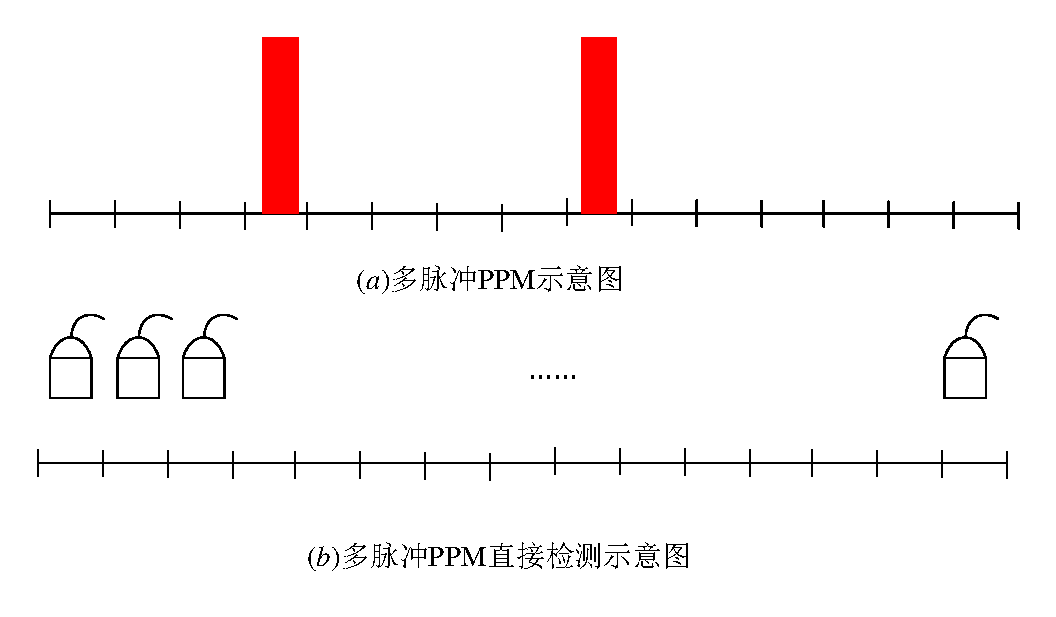
\includegraphics[width=0.8\textwidth]{figures/chap4/MPPM-DD}
  \caption{MPPM信号和直接检测示意图}
  \label{fig:MPPM-DD}
\end{figure}

在经典的光通信系统中,与PPM信号一样,采用直接检测的方法
对MPPM信号进行探测\cite{simon2003multi}。
直接检测探测方法利用一个ON-OFF探测器,
对每一个时隙进行独立的探测。
设每一个时隙的输出为$o_i$,如果有脉冲
$o_i=1$,否则$o_i=0$。
那么$M$个时隙对应的$M$个输出
构成输出序列$\bm{o} = (o_1,o_2,\cdots,o_M)$。
当所有的$M$个时隙都探测完毕,
然后通过最大似然准则进行译码判决\cite{simon2003multi}。
对于给定的码字$\bm{c}_i$,输出序列为$\bm{o}$的条件概率为
\begin{equation}
\Pr{\bm{o} | \bm{c}_i} = \prod_{k=1}^M \left(1 - e^{-c_{ik}n} \right)^{o_{k}} \left(e^{-c_{ik}n} \right)^{1-o_{k}} .
\end{equation}
其中$\bm{c}_i=(c_{i1},\cdots,c_{iM})$
和$\bm{o}=(o_{1},\cdots,o_{M})$
分别为码字和输出序列,
$n=|\alpha|^2$是一个脉冲的平均光子数。
最大似然准则通过计算对给定的输出序列$\bm{o}$
每一个符号对应的条件概率,
选择出条件概率最大的符号进行判决,
该条件概率也称似然函数。







\subsection{MPPM信号平方根检测极限}

\subsection{MPPM条件归零接收机}


\section{编码后OOK调制信号条件归零接收机}
\subsection{标准量子极限}

\subsection{编码后OOK调制信号平方根检测极限}

\subsection{编码后OOK调制信号条件归零接收机}



\section{编码后BPSK调制信号条件归零接收机}
\subsection{标准量子极限}

\subsection{编码后BPSK调制信号平方根检测极限}

\subsection{编码后BPSK调制信号条件归零接收机}


